%!TEX root = ../../template.tex
\section{Tomographic algorithms and reconstruction techniques}%
\label{sec:tomographic_algorithms_and_reconstruction_techniques}

Tomography is the cross-sectional imaging of an object through the use
of transmitted or reflected waves, captured by the object exposure to
the waves from a set of known angles. It has many different applications
in science, industry, and most prominently, medicine. Since the
invention of the Computed Tomography (\gls{CT}) machine in 1972, by
Hounsfield~\cite{Gunderman2006}, tomographic imaging techniques have had
a revolutionary impact, allowing doctors to see inside their patients,
without having to subject them to more invasive
procedures~\cite{Kak2001}.

The central thought around tomographic image reconstruction is to
recreate the information contained inside a target physical body,
without having to cut it or open it in any way. The theory is based on
Radon's idea that it is possible to "\emph{represent a function written
in $\mathbb{R}$ in the space of straight lines ($\mathbb{L}$) through
its line integrals}"~\cite{Radon1986}.

Say we have a body that we want to fully characterise without cutting
open or destroying in any way. Now imagine we can traverse it with some
kind of radiation, ray by ray, and that we are able to measure the rays
after they traverse the target. What we would capture would be relative
to the emitted radiation, of course, but it would also contain
information on how that ray had interacted with the target body's
matter. In the case of the ubiquitously used X-Ray radiation, the
measurement would be one of the total attenuation "imprinted" onto the
ray by the target body's molecules, in the ray's particular direction.
If said body is heterogeneous, the total attenuation can be derived by
the infinitesimal sum of all different attenuation phenomena caused by
the object's several different constituents (the same can be said of a
homogeneous object, but in that case there is only one type of
attenuation present). This means that each one of the rays contains
information regarding the constitution of said body.

The question that arises is thus "\emph{how we can use this information
to create a spatially accurate representation of this target's interior
composition?}". The answer to this question lies on many factors, but
the most prominent of which are surely choosing the quantity that we are
trying to find (that characterises the object) and assembling the
projections (that is what we call the line integrals in tomographic
imaging) in a way that allows solving an equation system for the
aforementioned quantity. This assembly, a matrix of projections
organised by their angles and position within the detector, is called
sinogram. All tomography methods revolve around finding the relationship
between it and the system's geometrical description~\cite{Bruyant2002,
Kak2001, Herman1973, Herman1995, Herman2009, Defrise2003}.

Let's consider the case in which we deal with a single ray of solar
light entering the atmosphere at a given point. Since the atmosphere
contains numerous absorbers and comparable atmospheric effects, the ray
changes from the point where it enters the atmosphere to the point at
which it is measured by a detector. Total absorption will depend on the
pollutant species, their cross-section and their concentration, since it
obeys Lambert-Beer's law. Looking from another angle, this absorption
is also the line integral that we will use to reconstruct our image.
With \gls{DOAS}, it is possible to measure several pollutants at the
same time, but for simplicity (and since it is one of the most studied
compounds in the field), let's consider that the single pollutant in our
atmospheric mixture is NO$_2$.

The problem of tomographic reconstruction can be approached in a number
of ways, depending mostly on the authors. In my literary search, I have
found that Kak and Slaney~\cite{Kak2001} have certainly explained this
problem in one of the clearer ways available. Therefore, I shall base
the rest of my presentation in their writings, and complement with other
authors' notes wherever necessary.

Considering the coordinate system displayed in
Figure~\ref{fig:coordinates}. In this schematic, the object is
represented by the function $f(x, y)$. The  $(\theta, t)$ parameters can
be used to define any line in this schematic. Line AB in particular can
be written:

\begin{equation}
    \label{eq:lineAB}
    x \cdot \cos(\theta) + y \cdot \sin(\theta) = t
\end{equation}

\begin{figure}[htpb]
    \centering
    \includegraphics[width=0.7\textwidth]{img/png/coordinates.png}
    \caption{Schematic representation for coordinate setting. The image
    depicts a parallel projection setting~\cite{Kak2001a}.}
    \label{fig:coordinates}
\end{figure}

And if we were to write a line integral along this line, it would look
like Equation~\ref{eq:lineABIntegral}, the Radon transform of function
$f(x, y)$:

\begin{equation}
    \label{eq:lineABIntegral}
    P_{\theta}(t) = \int_{-\infty}^{\infty} f(x, y) \cdot \delta(x \cdot
    \cos(\theta) + y \cdot \sin(\theta) - t) dxdy
\end{equation}

Where $\delta$, the delta function, is defined in
Equation~\ref{eq:delta}.

\begin{equation}
    \label{eq:delta}
    \delta (\phi) =  
    \begin{cases}
            1, & \phi = 0\\
            0, & otherwise
    \end{cases}
\end{equation}

As I have mentioned previously, a projection is a set of line integrals
such as $P_{\theta}(t)$. Geometry plays a very important role in how the
integrals are written and solved for reconstruction. The simplest case
is the one where the set is acquired in a row, describing what is called
a parallel geometry. Another more complex case is when a single point
source is used as origin for all rays, forming a fan. This is called a
fan-beam array. There are other possible geometries, but they fall out of
the scope of this work and will therefore not be addressed any further.

The Fourier Slice Theorem (\gls{FST}) is the most important component of
the most important algorithm in tomographic inversion, the Filtered
BackProjection algorithm (\gls{FBP}). \gls{FST} is based on the equality
relation between the 
two-dimensional Fourier Transform (\gls{FT}) of the object function and
the one-dimensional \gls{FT} of the object's projection at an angle
$\theta$. Let's start by writing the 2D \gls{FT} for the object
function, Equation~\ref{eq:objectFT}, and the 1D \gls{FT} of projection
P$_\theta$, in Equation~\ref{eq:1dFTproj}.

\begin{equation}
    \label{eq:objectFT}
    F(u, v) = \int_{-\infty}^{\infty} \int_{-\infty}^{\infty} f(x, y)
    \cdot \exp \left [ -j2\pi (ux + vy) \right ] dx dy 
\end{equation}

\begin{equation}
    \label{eq:1dFTproj}
    S_{\theta}(\omega) = \int_{-\infty}^{\infty} P_{\theta} \cdot \exp\left[
    -j2 \pi \omega t \right]
\end{equation}

For simplicity, let's consider the 2D \gls{FT} at the line defined by
$v=0$ in the frequency domain. We rewrite the 2D \gls{FT} integral as:

\begin{equation}
    \label{eq:v0}
    F(u, 0) = \int_{-\infty}^{\infty} \int_{-\infty}^{\infty} f(x, y)
    \cdot \exp \left[  -j 2\pi  \omega ux \right] dx dy
\end{equation}

Notice that $y$ is not present in the phase factor of the \gls{FT}
expression anymore, and this means we can rearrange the integral as:

\begin{equation}
    \label{eq:v02}
    F(u, 0) = \int_{-\infty}^{\infty} \left[ \mathbf{\int_{-\infty}^{\infty}
    f(x, y) dy }\right] \cdot \exp \left[  -j 2\pi  \omega ux \right] dx 
\end{equation}

Now, the \textbf{bold} part of Equation~\ref{eq:v02} is similar to
Equation~\ref{eq:lineABIntegral}. It is precisely that equation,
considering $\theta=0$ and a constant value of $x$, as in
Equation~\ref{eq:p0}.

\begin{equation}
    \label{eq:p0}
    P_{\theta=0} (x) = \int_{-\infty}^{\infty} f(x, y) dy
\end{equation}

This in turn can be substituted in Equation~\ref{eq:v02}, finally
arriving at:

\begin{equation}
    \label{eq:FTP}
    F(u, 0) = \int_{-\infty}^{\infty} P_{\theta=0} (x) \cdot \exp \left[
    -j 2\pi ux \right] dx
\end{equation}

And this is the one-dimensional \gls{FT} for the projection at angle
$\theta=0$. Finally, the enunciation of the Fourier Slice Theorem:
\begin{center}
    \begin{minipage}{0.8\textwidth}

        \noindent\textbf{\emph{The Fourier Transform of a parallel
                projection  of an image $f(x, y)$ taken at angle
                $\theta$ gives a slice of the two-dimensional Fourier
                Transform, $F(u, v)$, subtending an angle $\theta$ with
                the $u$-axis (see Figure~\ref{fig:fst})}}

    \end{minipage}
\end{center}

\begin{figure}[htpb]
    \centering
    \includegraphics[width=.8\textwidth]{img/png/fst.png}
    \caption{The \gls{FST}, a schematic
    representation~\cite{Asl2013a}.}
    \label{fig:fst}
\end{figure}

If one takes the \gls{FST} into account, the idea behind the \gls{FBP}
seems to appear almost naturally. Say one has a single projection and
its Fourier transform. From the \gls{FST}, this projection is the same
as the object's two-dimensional \gls{FT} in a single line. A crude
reconstruction of the original object would result if someone were to
place this projection in its right place in the Fourier domain and then
perform a two-dimensional \gls{IFT}, while assuming every other
projection to be 0. The result, in the image space, would be as if
someone had smeared the object in the projections direction.

What is really needed for a correct reconstruction is to do this many
times, with many projections. This brings a problem with the method:
smearing the object in all directions will clearly produce a wrong
\emph{accumulation} in the center of the image, since every projection
passes through the middle (remember we are still talking about parallel
geometry projections) and are summed on top of each other, but on the
outer edges, this does not occur. If one does not address this, the
image intensity levels in the reconstructed image will be severely
overestimated in the center and underestimated in the edges (due to
normalization). The solution is conceptually easy: we multiply the
Fourier transform by a weighting filter proportional to its frequency
($\omega$) and that encompasses its relevance in the global scheme of
projections. If there are $K$ projections, then it is adequate for this
value to be $\frac{2\pi\lvert\omega\rvert}{K}$. As an algorithm,
\gls{FBP} can be written as in Algorithm~\ref{alg:fbp}.

\begin{algorithm}
    \caption{The Filtered BackProjection Algorithm}
    \label{alg:fbp}
    \SetAlgoLined
    \KwResult{A reconstructed image of the projected object.}
    \For{$\theta \gets 0$ \KwTo $180$ \KwBy $\frac{180}{K}$}{
        measure projection $P_{theta}(t)$\;
        FT($P_{\theta}(t)$), rendering $S_{\theta}(\omega)$\;
        Multiply by $\frac{2\pi\lvert{\omega}\rvert}{K}$\;
        Sum the \gls{IFT} of the result in the image space\;
    }
    
\end{algorithm}

Parallel projections, in which the object is scanned linearly from
multiple directions, have the advantage of having a relatively simple
reconstruction scheme. However, they usually result in acquisition times
which are in the order of minutes. A faster way of collecting the data
is one where all radiation emanates from a single point-source, which
rotates around the target object (as well as the detectors). There are
two types of fan-beam projections: equiangular and equally spaced. In
this project, I have only worked with equiangular processes, so I will
not include an explanation for equally spaced fan-beam projections. The
reader may find this well described (much better than I would be able
to) in ~\cite{Kak2001} and ~\cite{Herman1973}.

Consider Figure~\ref{fig:equiangular}. If our projection data were
acquired through a parallel ray geometry, we would be able to say that
ray SA belonged to a projection $P_{\theta}(t)$, in which $\theta$ and
$t$ would be written:

\begin{equation}
    \label{eq:theta_and_t}
    \theta = \beta + \gamma \quad \text{ and } \quad t = D \cdot \sin \gamma
\end{equation}

In Equation~\ref{eq:theta_and_t}, $D$ is the distance between the source
$S$ and the origin $O$; $\gamma$ is the angle of a ray within a fan and
$\beta$ is the angle that the source $S$ makes with a reference axis.
Through these relationships one can \emph{translate} the parallel
projection's \gls{FBP} algorithm to the fan-beam case, which involves several
complex geometric transformations, although the overall rationale is
exactly the same.

\begin{figure}[htpb]
    \centering
    \includegraphics[width=.8\textwidth]{img/png/fig319.png}
    \caption{Schematic representation of an equiangular fan-beam
    projection, taken from~\cite{Kak2001}.}
    \label{fig:equiangular}
\end{figure}

Another particularity of fan-beam projection data is the fact that they
can be sorted into a parallel projection. For that, one starts with the
premise that if one were to substitute the fan geometry for parallel
beams, most of the fan-beam rays would also appear in some projection of
the parallel setup. This re-sorting algorithm starts with
Equation~\ref{eq:theta_and_t}. Now, if we call a fan-beam projection
taken at angle $\beta$ $R_{\beta}(\gamma)$, and a parallel projection
taken at angle $\theta$ $P_{\theta}(t)$, one could thus write
Equation~\ref{eq:parallel_vs_fanbeam}, which can already be used to
re-sort any fan-beam projection into parallel beam geometry.

\begin{equation}
    \label{eq:parallel_vs_fanbeam}
    R_{\beta}(\gamma) = P_{\beta + \gamma}(D \cdot \sin \gamma)
\end{equation}

The angular interval between fan-beam projections can be written
$\delta\beta$, and the angular interval of rays within each fan is
written $\delta\gamma$. In the case that they are the same
($\beta=\gamma=\alpha$), then it it is the case that they can both be
replaced by multiples of that interval in
Equation~\ref{eq:parallel_vs_fanbeam}, which becomes
Equation~\ref{eq:parallel_vs_fanbeam2}.

\begin{equation}
    \label{eq:parallel_vs_fanbeam2}
    R_{m \cdot \alpha}(n \cdot\alpha) = P_{m \cdot\alpha + n
    \cdot\alpha}(D \cdot \sin n \cdot\alpha)
\end{equation}

Or, in non-mathematical notation, the n\textsuperscript{th} ray of the
m\textsuperscript{th} radial projection (R) is the same as the
n\textsuperscript{th} ray in the (m+n)\textsuperscript{th} parallel
projection. Although being much simpler than directly applying the
\gls{FBP} algorithm to the fan-beam projection data, this method has a
limitation, which is the non-uniformity of the generated parallel
projections. This can usually be corrected through
interpolation~\cite{Kak2001a}. 

\subsection{Iterative Tomographic Reconstruction Methods}%
\label{sub:theobg_tomography_iterativemethods}

This subsection borrows heavily from an article I published in 2021, in
which I described the tomographic part of this
thesis~\cite{ValentedeAlmeida2020}.  

Iterative reconstruction algorithms are based on simpler premises than
\gls{FBP}, but they do require a more computational approach. One can
start by thinking that a certain tomographic problem is modelled by its
sinogram, which is the set of all projections that were gathered by the
sensors. The sinogram is a matrix whose columns represent the sensor
that gathered the information and whose lines represent the projection
number. The resulting image can also be thought of as a matrix. Each
value of this matrix corresponds to a pixel intensity, which gives it
its intensity and/or colour. The third matrix is the system matrix. This
matrix stores the length of each ray in each projection contained in one
of the image's pixels. These lengths are obtained through a process
called discretisation. One of the most famous and studied algorithms for
this purpose (and the one I ended up using for this work), the Siddon
algorithm, is described some paragraphs ahead, in
Section~\ref{sub:theobg_tomography_iterativemethods_siddon}.

Iterative methods attempt to solve the relationship between these three
matrices, which is presented in Equation~\ref{eq:iterative_general}. In
it, $\mathbf{g}\in\mathbb{R}^{m, 1}$ is the column vector sinogram,
$\mathbf{a} \in \mathbb{R}^{m,n}$ is the system matrix and $\mathbf{f}
\in \mathbb{R}^{n, 1}$ is the column vector image. $m$ is the number of
measurements (projections times detectors) and $n$ is the number of
pixels in the image. As their designation implies, iterative algorithms
produce an estimation for $\mathbf{f}$ which is updated in the direction
of error minimisation in every iteration~\cite{Kak2001, Bruyant2002}.

\begin{equation}
    \centering
    \mathbf{g} = \mathbf{a} \cdot \mathbf{f}
    \label{eq:iterative_general}
\end{equation}

The popularity of algebraic reconstruction methods has not remained
constant throughout the years. For a long time, they have been
considered too computationaly intensive to use in a clinical setting
(paradoxically, Hounsfield's machine used this kind of algorithm). This
was in direct opposition to the fact that researchers know that these
methods are better able to model reconstruction since Shepp and Vardi
published the maximum likelihood tracer estimation in 1982. Nowadays,
and since the mid nineties, these algorithms are the first choice
whenever the reconstruction dataset is not too large to process using
the available computational capabilities~\cite{Defrise2003}.

The general goal of iterative reconstruction algorithms is to solve
Equation~\ref{eq:iterative_general}~\cite{Bruyant2002a}. In principle,
any method that solves it can be used for image reconstruction in
tomography. In reality, however, only a few are currently in use by the
community. Of these, TomoSim uses two of the most prominent:
Simultaneous algebraic Reconstruction Technique (SART) and Maximum
Likelihood Expectation Maximisation (MLEM). 

SART was presented in 1984 by Andersen and Kak~\cite{Andersen1984a} and
the global idea is that the estimated image is corrected for all
projections at the same time (in opposition to the original algebraic
Reconstruction Technique, in which corrections were applied for each
single projection). Iterations in SART change the estimated image
according to Equation~\ref{eq:sart}, iterating on $k$.

\begin{equation}
    \centering
    \mathbf{g}_{i}^{(k+1)} = \mathbf{g}_{i}^{(k)} + \frac{\sum_j \left[
            \mathbf{a}_{ij} \cdot \frac{p_{j} - \mathbf{a}_{j}^{T} \cdot
    \mathbf{g}^{(k)}}{\sum_{i=1}^{n}\mathbf{a}_{ij}}\right]}{\sum_j
    \mathbf{a}_{ij}}
    \label{eq:sart}
\end{equation}

MLEM algorithms were first published in the medical imaging community in
1982, by Shepp and Vardi~\cite{Shepp1982}. With this algorithm, image
corrections are ruled by Equation~\ref{eq:mlem}, which also iterates
over $k$.

\begin{equation}
    \centering
    \mathbf{f}_{j}^{k + 1} =
    \frac{\mathbf{f}_{j}^{k}}{\sum_{i=1}^{n}\mathbf{a}_{ij}}
    \sum_{i=1}^{n}\frac{\mathbf{g}_i}{\sum_{j'=1}^{m}\mathbf{a}_{ij'}\mathbf{f}_{j'}^{k}}
    \label{eq:mlem}
\end{equation}

This equation is very easy to implement computationally, if one observes
that the sums of the second multiplication term expand neatly onto
matrix products. In the end, this equation is the equivalent of writing
Equation~\ref{eq:mlem_simplified}, as explained in~\cite{Bruyant2002a},
in which IMG$^{(k)}$ is the estimated image in the k$^{\text{th}}$
iteration, NBP is the Normalised Backprojection operation, RSNG the real
sinogram (as in coming from the detector hardware) and SSNG the
simulated sinogram, calculated through the previous iteration.

\begin{equation}
    \centering
    \begin{split}
        \text{IMG}^{(k+1)} = \text{IMG}^{(k)}&
        \times\text{NBP} \left(\frac{\text{RSNG}}{\text{SSNG}^{(k)}}\right)
    \end{split}
    \label{eq:mlem_simplified}
\end{equation}


\subsection{Discretisation - The Siddon Algorithm}%
\label{sub:theobg_tomography_iterativemethods_siddon}

Discretisation is the process by which the \gls{ROI} is digitised into a
computational platform. There are several algorithms designed for this
effect that are available in the literature. One of the easiest to
implement that is also adequate to this application (unsurprisingly)
comes from the medical imaging field. It was published in 1985 by Robert
Siddon~\cite{Siddon1985}.

The Siddon algorithm is one of the foremost path calculation algorithms
in the medical field of radiology. It is not only used for the
discretisation of tomographic fields, but also in the dose calculation
process of radiation therapy patients. The idea behind the algorithm is
that the total dose of a radiation ray, i.e., its path, is given by the
sum of the length within each pixel that this ray traverses multiplied
by the density of said pixel. In mathematical notation, one can write
this as in Equation~\ref{eq:siddon_sum}.

\begin{equation}
    \label{eq:siddon_sum}
    d = \sum_{i}\sum_{j}\sum{k} l(i, j, k)\cdot\rho(i, j, k)
\end{equation}

In Equation~\ref{eq:siddon_sum}, $d$ is the radiological path (the
projection value), $i$, $j$, $k$ are the coordinate vectors, $l$ is the
length within a pixel and $\rho$ is the pixel density. In our case, this
last value is the trace gas column density for that pixel.

The main reason for Siddon's algorithm being easy to implement is its
treatment of pixels (or voxels if in 3D). Instead of considering pixels
as \emph{atomic}\footnote{In their undivisible sense.} units, it defines
them as the intersections of orthogonal sets of equally spaced lines
(planes in 3D). Pixel lengths are determined by the looking at the
intersections between the orthogonal lines and the radiation ray. 

\begin{figure}[htpb]
    \centering
    %\includegraphics[trim=left bottom right top, clip]{file}
    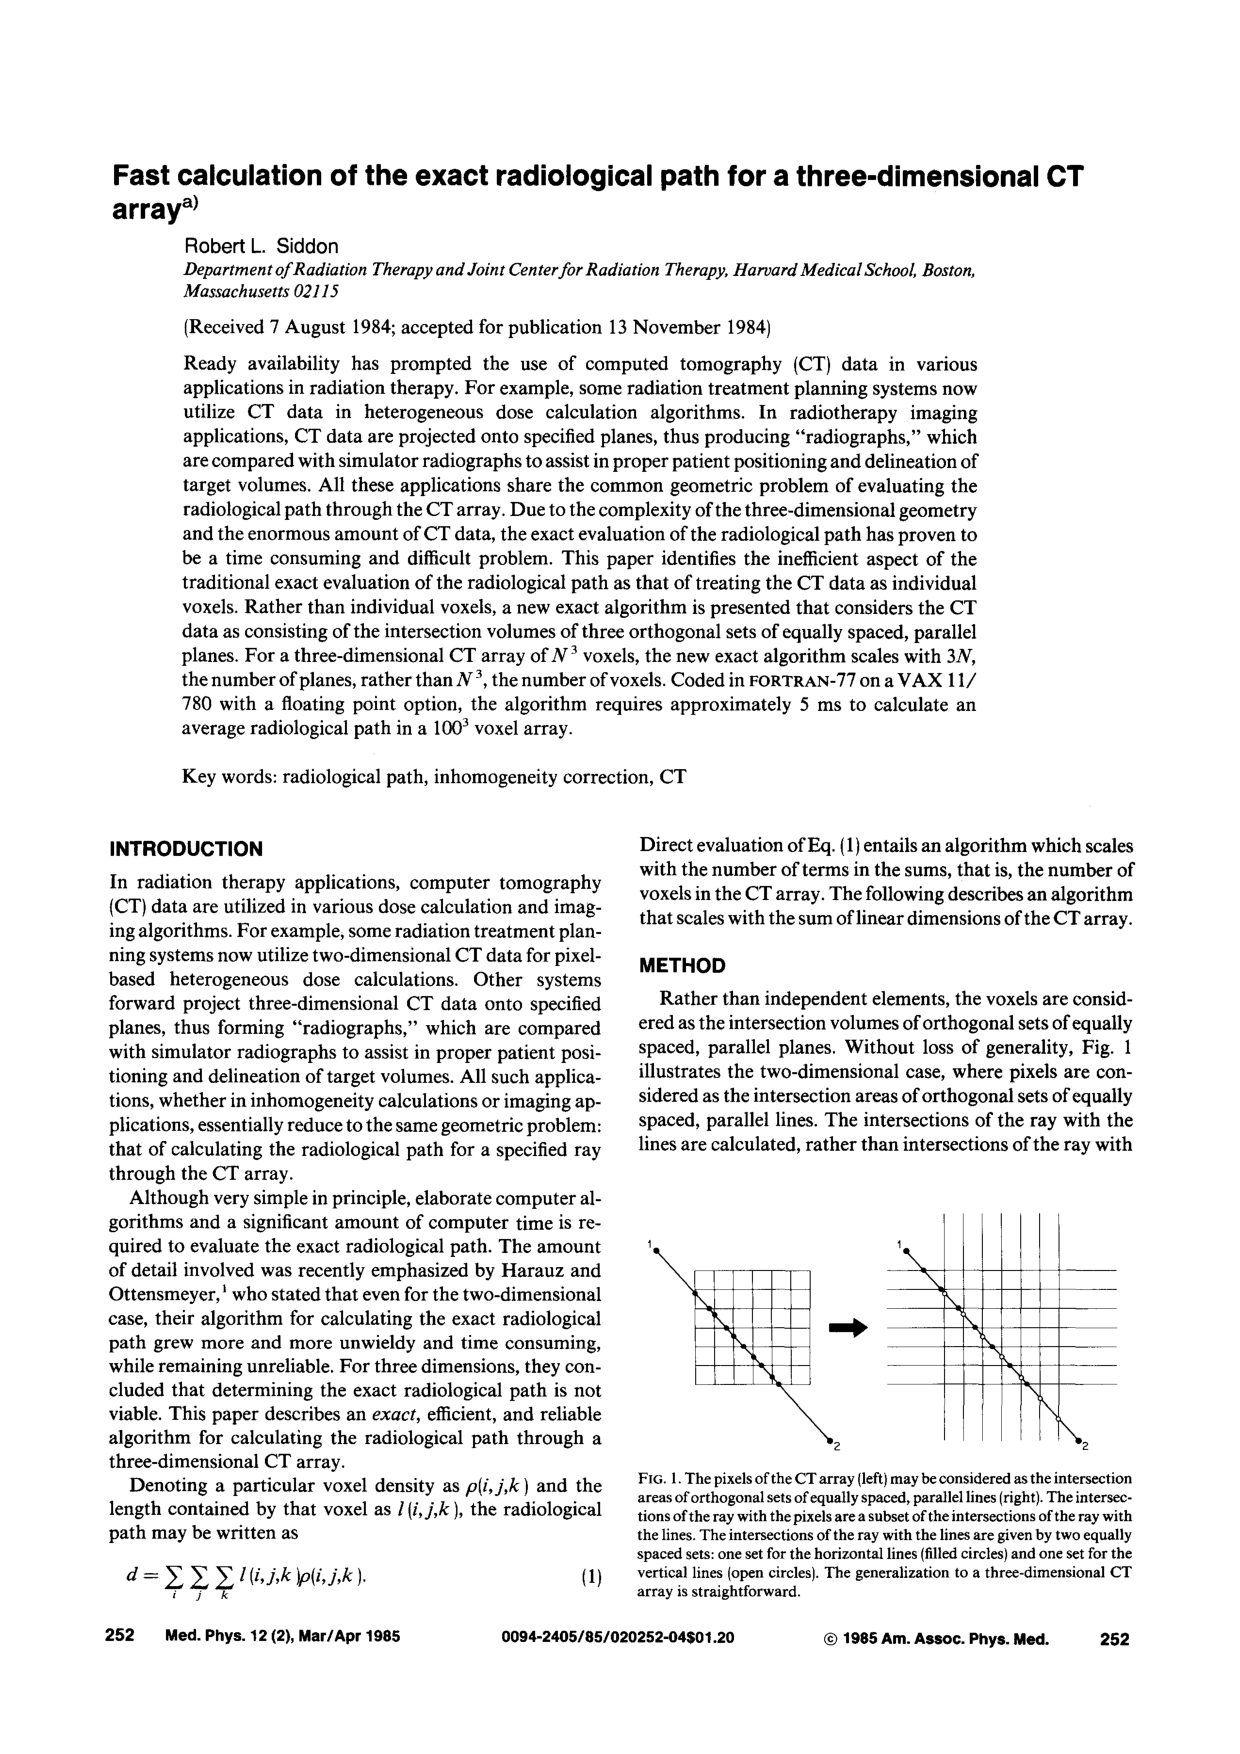
\includegraphics[trim=11cm 5cm 2cm 20cm, clip]{img/pdf/siddon_pg1.pdf}
    \caption{Grid and pixel definition, as they appear in the original
        article by Robert Siddon~\cite{Siddon1985}.  Pixels are "formed"
        by intersecting the ray (here going from point 1 to point 2)
        with the superimposed grid.}
    \label{fig:siddon_pixels}
\end{figure}

Since lines are orthogonal and equally spaced, all intersections can be
calculated recursively after knowing where the first intersection is
located. The calculation of the radiologic path is achieved by
determining the subset of the intersections between the orthogonal lines
and the lih+ght ray that identifies individual pixels.

If $P_1 \to (X_1, Y_1)$ and $P_2 \to (X_2, Y_2)$ are the start and
end of the radiologic path within the \gls{ROI}, the line between them
can be parametrically written as in Equation~\ref{eq:p1p2parametric}.

\begin{equation}
\label{eq:p1p2parametric}
    \begin{aligned}
        X(\alpha) = &X_1{} + \alpha \cdot (X_2 - X_1)\\
        Y(\alpha) = &Y_1{} + \alpha \cdot (Y_2 - Y_1)
    \end{aligned}
\end{equation}

In Equation~\ref{eq:p1p2parametric}, $\alpha$ is 0 at $P_1$ and 1 at
point $P_2$. Values of $\alpha$ within the \gls{ROI} vary according to
the positions of $P_1$ and $P_2$ with respect to the \gls{ROI}. By
determining $\alpha$ values of each intersection (in both directions),
one can determine the length of the ray within the pixel by the
difference of adjacent intersections. The whole algorithm can be written
as in Algorithm~\ref{alg:siddon}.

\begin{algorithm}[H]
\SetAlgoLined
\KwResult{Discretised ROI space.}
calculate range of parametric values\;
calculate range of pixel indices\;
calculate parametric sets\;
merge sets\;
calculate pixel(or voxel) lengths\;
calculate pixel indices\;
\caption{Siddon's algorithm's procedural steps. After running this
algorithm, one is able to represent any continuous ray through the
analysis field as a sum of discrete lengths}
\label{alg:siddon}
\end{algorithm}

Detailing the two-dimensional case\footnote{A
three-dimensional case would be just the same but with an additional
coordinate.} should start by the definition of the discretisation grid
itself, as in Equation~\ref{eq:discretisation_grid}. The equation
reflects the recursive nature of the grid definition. In it, $d_x$ and
$d_y$ are the distances between the $x$ and $y$ planes, which correspond
to the lengths of the pixels in those coordinates. $N_x$ and $N_y$ are
the number of pixels in $x$ and $y$ that are contained in the grid.

\begin{equation}
    \label{eq:discretisation_grid}
    \begin{aligned}
        X_{plane}(1) &= X_{plane}(1) + (i-1) \cdot d_x\\
        Y_{plane}(1) &= Y_{plane}(1) + (j-1) \cdot d_y\\
    \end{aligned}
\end{equation}

The parametric values $\alpha_{min}$ and $\alpha_{max}$ are given by the
intersections of the ray with the sides of the grid ($i = 1$ and $i =
N_x$) and can be written as in Equation~\ref{eq:alpha_limits}.

\begin{equation}
    \label{eq:alpha_limits}
    \begin{aligned}
        \alpha_{min} &= max \left\{  0, min \left[  \alpha_x(1),
                \alpha_x(N_x)  \right], min\left[ \alpha_y(1),
                    \alpha_y(N_y)  \right] \right\}\\
        \alpha_{max} &= min\left\{ 1, max\left[ \alpha_x(1),
                \alpha_x(N_x)  \right], max\left[ \alpha_y(1),
                    \alpha_y(N_x) \right]  \right\}\\
    \end{aligned}
\end{equation}

Not all line intersections have a corresponding parametric value. The
ones that do are comprised within index ranges that are defined by
Equation~\ref{eq:parametric_ranges}. This equation presents the case for
the first coordinate ($x$), with the second coordinate having an
identical expression.

\begin{equation}
    \label{eq:parametric_ranges}
    \begin{aligned}
        i_{min} &= N_x - \frac{ X_{plane}(N_x) - \alpha_{min}(X_2 - X_1)
            - X_1 }{d_x}\\
        i_{max} &= 1 + \frac{X_1 + \alpha_{max}(X_2 - X_1) -
            X_{plane}(1)}{d_x}\\
    \end{aligned}
\end{equation}

Equation~\ref{eq:parametric_ranges} defines a range of possible indices
for the pixels, in parametric fashion. We can use this range to
construct the set of used parametric indices, given in
Equation~\ref{eq:parametric_index_set} for the $x$ coordinate. 

\begin{equation}
    \label{eq:parametric_index_set}
    \left\{ \alpha_x \right\} = \left\{ \alpha_x(i_{min}), \ldots,
        \alpha_x(i_{max})  \right\}
\end{equation}

Although Equation~\ref{eq:parametric_index_set} only presents the
expression for the first coordinate, there are similar expressions for
the other coordinates at play. After determining the set of possible
indices for $x$ and $y$, these sets must be arranged in ascending order,
creating an index superset. To this the minimum and maximum values,
calculated in Equation~\ref{eq:alpha_limits}, are appended. The
resulting and final set of parametric values is presented in
Equation~\ref{eq:final_parametric_set}.

\begin{equation}
    \label{eq:final_parametric_set}
    \begin{aligned}
        \alpha^* &= merge(\alpha_x, \alpha_y)\\
        \{ \alpha \} &= \{ \alpha_{min}, \alpha^*, \alpha_{max} \}\\
                     &= \alpha(0), \ldots, \alpha(n)\\
    \end{aligned}
\end{equation}

Where the last term, $n$, is given by the sum of all index range
numbers, as in Equation~\ref{eq:n}, again for the two-dimensional case.

\begin{equation}
    \label{eq:n}
    n = (i_{max} - i_{min} + 1) + (j_{max} - j_{min} + 1)
\end{equation}

Each element of the array defined in
Equation~\ref{eq:final_parametric_set} is an intersection between the
ray and a given pixel. Since they are ordered, it is possible to
calculate the array of pixel lengths for each ray, using the expression
in Equation~\ref{eq:length1}.

\begin{equation}
    \label{eq:length1}
    l_{m} = d_{12}[ \alpha(m) - \alpha(m-1)] \quad (m = 1 \ldots n)
\end{equation}

With $d_{12}$ being the distance between $P_1$ and $P_2$, calculated
through the Euclidean formula for distance between two points. In
Tomosim, this distance is always equal to the trajectory's diameter.

Pixel $[i(m), j(m)]$ is located in the midpoint between the
m\textsuperscript{th} and the (m-1)\textsuperscript{th} intersections.
It is given by the expression in Equation~\ref{eq:pixel_pair}.

\begin{equation}
    \label{eq:pixel_pair}
    \begin{aligned}
        \alpha_{mid} &= \frac{\alpha(m) + \alpha(m-1)}{2}\\
        i(m) &= 1 + \frac{X_1 + \alpha_{mid}\cdot(X_2 - X_1) -
            X_{plane}(1)}{d_x}\\
        j(m) &= 1 + \frac{Y_1 + \alpha_{mid}\cdot(X_2 - X_1) -
            Y_{plane}(1)}{d_y}\\
    \end{aligned}
\end{equation}

And with this we are armed with all possible knowledge on the system's
geometry. Now let's integrate everything and gather our thoughts:
\begin{itemize}
    \item Tomographic imaging is the set of techniques with which we can
        create the image of an object by using said object's projection
        data;
    \item Projections are line integrals. They capture how a target body
        interferes with some kind of known radiation along a given
        line, which constitutes a ray;
    \item Projections are always indexed to an emitter and a receiver,
        which have perfectly determined positions;
    \item With the positions of the emitters, the \gls{ROI} grid and the
        Siddon algorithm, we can determine how exactly is each \gls{ROI}
        pixel traversed by each one of the rays;
    \item Summing all the lengths of all the pixels traversed by
        each ray gives us the optical path of said ray;
    \item Multiplying the length of a ray within a pixel with that
        pixel's density gives us how that particular pixel interferes
        with the radiation;
    \item A projection (remember, a line integral) can be approximated
        by the sum of all these individual contributions by particular
        pixels - and this is exactly what is meant by
        Equation~\ref{eq:siddon_sum}.
\end{itemize}

So here we have it. The last piece of the puzzle proposed by
Equation~\ref{eq:iterative_general}. The discretisation process, namely
Siddon's algorithm, allows us to determine the system matrix,
$\mathbb{a}$ in this equation. 
